%	Vorlage FAU



\documentclass[11pt,a4paper]{scrartcl}

\usepackage[utf8]{inputenc}				%Sonderzeichen als utf8@gedit und texmaker. sonst: latin1
\usepackage[T1]{fontenc}				%Europ. Zeichensatzkodierung, u.a. Umlaute
\usepackage{graphicx}					%Graphiken einbinden
\usepackage{lmodern}					%Verbesserte Schriftqualität
\usepackage[ngerman]{babel}				%neue deutsche Rechtschreibung
\usepackage{wrapfig}					%Graphiken umfließen		
\usepackage{multirow}					%Spezielle Tabellenfunktionen
\usepackage{amsmath}                    %Mathematische Bibliothek
\usepackage{setspace}
\usepackage[hmargin=3cm,vmargin=3.5cm]{geometry}

%Farbfunktionen
\usepackage{xcolor}							%Package

\definecolor{ltgray}{rgb}{0.95, 0.95, 0.95}	%Definition gray (Quellcode Hintergrund)
\definecolor{ltblue}{rgb}{0, 0.1, 1}		%Definition blue (Quellcode Identifier)
\definecolor{ltdred}{rgb}{0.8, 0.0, 0.25}   %Definition dunkel rot (Quellcode Strings)
\definecolor{ltgreen}{rgb}{0, 0.6, 0}		%Definition green (Quellcode def. Konstanten)
\definecolor{ltgray2}{rgb}{0.1, 0.1, 0.1}	%Definition dunkelgrau (Quellcode Kommentare)
\definecolor{ltpurple}{rgb}{0.5, 0, 0.7}	%Definition lila 

%Hyperlink Formatierung				
\usepackage[colorlinks=false,				%Text nicht farbig
			urlbordercolor={0 0 1},			%URLs blau
			linkbordercolor={1 1 1},		%interne Links weiß 
			pdfborderstyle={/S/U/W 1}]		%Links unterstrichen
			{hyperref}					

%Formatierung von Quellcode
\usepackage{listings}								%Package

\lstset{											%Befehl zum Parameter setzen
language=python,									%Visual(default) C++							
basicstyle=\small\ttfamily,							%Listing small
backgroundcolor=\color{ltgray}, 					%Hintergrundfarbe Hellgrau							
keywordstyle=\bfseries,								%Keywords fettgedruckt
identifierstyle=\color{ltblue},						%Identifier blau							
commentstyle=\color{ltgray2},						%Kommentare 
stringstyle=\itshape\color{ltdred},					%Strings dunkelrot
showstringspaces=false,								%keine speziellen String spaces
numbers=left,										%Zeilennummerierung links
numbersep=15pt,										%Abstand zwischen Zeilennummern und Quellcode
xleftmargin=30pt,									%Abstand Zeilennummern zu Rand
emph={LCD_LINE1, LCD_LINE2, LCD_LINE3, LCD_LINE4, 	%Definition von Konstanten
LCD_LINE5, LCD_LINE6, LCD_LINE7, LCD_LINE8, 
OUT_A, OUT_B, OUT_C, OUT_AB, OUT_AC, OUT_BC, 
S1, S2, S3, S4, IN_1, IN_2, IN_3, IN_4},
emphstyle=\color{ltgreen},							%Konstanten grün
literate=											%ermöglicht Umlaute in listings
{Ö}{{\"O}}1
{Ä}{{\"A}}1
{Ü}{{\"U}}1
{ß}{{\ss}}2
{ü}{{\"u}}1
{ä}{{\"a}}1
{ö}{{\"o}}1
} 						


% ------ Formatierung Kopf- und Fußzeile
\usepackage{scrpage2}							%Package

\pagestyle{scrheadings}
\clearscrheadings
\clearscrplain

\lohead{Seminararbeit Textmining}
\cohead{}
\rohead{FAU Erlangen}
\lofoot{}
\cofoot{}
\rofoot{\pagemark}
\setheadsepline{0pt} 							%Keine Linie für Kopfzeile
\setfootsepline{0pt} 							%Keine Linie für Fußzeile
%--------------------------------



% --------- Formatierung Titelseite --------- %
\newcommand{\Titelseite}{

\begin{titlepage} 

\pagestyle{empty}

%Kopf
\begin{minipage}[t]{6cm}
\vspace{0pt}	
\Kurs 															%Kursname
\end{minipage}
\hfill
\begin{minipage}[t]{4cm}
\vspace{-20pt}							

\includegraphics[scale=0.20]{images/logo.png} 				%rechtsbündiges Logo
\end{minipage}														
	
	
%Mitte
\begin{center}

\vspace{3cm}
\begin{doublespace}
\textbf{\Huge \Titel} \\[2.5cm]									%Titel
\end{doublespace}

\begin{large}

Autor: \Autor \\[0.5cm]                                                %Autor
Matrikelnummer: 21889343 \\[1cm]
\Datum \\[1.5cm]												%Datum
%Version: \Version \\[1cm]										%Version
letzte Aktualisierung: \today \\[2cm]							%Aktualisierung


%Fuß
Friedrich-Alexander-Universität Erlangen-Nürnberg\\
Department Informatik

\end{large}

\end{center}				

\thispagestyle{empty}											%unterdrückt Seitennummer

\end{titlepage}

}

% ---------------------------------------- %



% -------- Individuelle Anpassung -------- %

%Kurs
\newcommand{\Kurs}{Seminar Textmining}
%Titel
\newcommand{\Titel}{Klassifikation von Dokumenten nach Themen}
%Autor: Professoren, Studentenn, etc				
\newcommand{\Autor}{Simon Hofmann}
%Datum
\newcommand{\Datum}{14.06.2015}		
%Version
%\newcommand{\Version}{V1.0}

\DeclareMathOperator*{\argmin}{arg\,min}
\DeclareMathOperator*{\argmax}{arg\,max}

% -------- Anmerkung zum Einfügen von Graphiken ----------- % 


% Syntax: 
% \includegraphics[Optionen]{Pfad/Dateiname}

%	 Als Optionen sind folgende Formatierungen verfügbar:

% 		angle - Bestimmt den Drehwinkel um einen Referenzpunkt für die Grafik. Positive Werte drehen die Grafik 
% 				gegen den  Uhrzeigersinn, negative mit ihm. 

% 		draft - Ist draft gesetzt, wird nur ein Platzhalter der Grafik angezeigt. Beschleunigt den Übersetzungsvorgang 
% 				des Dokuments erheblich. Oftmals kann draft auch in den Dokumentoptionen angegeben werden. 

% 		scale - Skaliert die Grafik anhand eines Skalierungsfaktors. 

% 		height - Skaliert die Grafik auf die angegebene Höhe. Die Angabe der Größe muss in einer LaTeX-spezifischen 	%				 Einheit  erfolgen. 

% 		width - Skaliert die Grafik auf die angegebene Breite. Die Angabe der Größe muss in einer LaTeX-spezifischen 	%				Einheit erfolgen. 
	


% Um die Platzierung der Grafik Latex zu überlassen muss sie in eine figure-Umgebung eingebunden werden:

%		\begin{figure}[Parameter]
%		\includegraphics{Dateiname.eps}
%		\caption{Titel der Grafik}				Beschriftung der Grafik
%		\label{labelname}						Falls die Grafik intern verlinkt werden soll
%		\end{figure}

%	Als Parameter sind verfügbar:

%    h (here): Platziere die Grafik möglichst dort, wo der Befehl zur Einbindung steht.
%    t (top): Platziere die Grafik möglichst am Anfang einer Seite.
%    b (bottom): Platziere die Grafik möglichst am Ende einer Seite.
%    p (float page): Platziere die Grafik möglichst auf einer Seite, die nur "floating"-Objekte enthält.

% Beispiel:

%	\begin{figure}[htbp]
%		\centering
%			\includegraphics[scale=0.3]{images/Robo.jpg}
%			\label{fig:Roboter}
%			\caption{Roboter}		
%	\end{figure}

% -------------------------------------------------------------------- %

% ----- Quellcode einbinden ---------%

%	Um Latex die Formatierung von Quellcode zu ermöglichen muss der Code einfach in die folgenden Anweisungen  
%   eingebunden werden

%	\begin{lstlisting}
%	<Quellcode>
%	\end{lstlisting}


%Beginn Dokument
\begin{document}
							
\Titelseite									%erstellt Titelseite

%Inhaltsverzeichnis
\thispagestyle{empty}
\tableofcontents

\newpage
\setcounter{page}{1}						%Nach Titelseite beginnt das Dokument mit Seite 1
\setcounter{section}{0}

%Hier .tex file importieren
\section{Einleitung}
    Die automatische Klassifikation von Dokumenten spielt in der modernen Welt eine tragende Rolle. 
    Wegen des rasanten Wachstums an Informationen im Internet ist es notwendig, Dokumente bezüglich ihrer Art oder ihres Inhalts in Kategorien zu unterteilen, um effiziente Suchen zu ermöglichen. 

    Einen großen Anwendungsbereich stellt auch der tägliche Umgang mit Diensten wie zum Beispiel Email dar, bei der eine Klassifikation von Text unabdingbar ist, um wichtige Nachrichten von unnötiger Werbung zu trennen (Spam-Filterung).
    Ebenso ist es möglich, den eigenen Posteingang automatisch nach Kategorien sortieren zu lassen~\cite{IIR}.

    Eine weitere mögliche Nutzung von Klassifikatoren ist die Filterung von Nachrichten, um dem Nutzer nur für ihn ``interessante'' Nachrichten zu präsentieren. 
    In~\cite{PersoNews} wurde ein solches System implementiert.\\

    Ziel dieser Arbeit ist es, die automatische Klassifikation von Textdokumenten nach Themen mit Hilfe eines naiven Bayes-Klassifikators zu erarbeiten.

    Kapitel 2 behandelt dazu die Grundlagen der Bayesschen Statistik, welche auch im naiven Bayes-Klassifikator zur Anwendung kommen. 

    Die theoretischen Hintergründe und Prinzipien des Klassifikators werden in Kapitel 3 behandelt, bevor in Kapitel 4 dann eine Implementierung der theoretischen Grundlagen genauer betrachtet wird sowie auf die weiteren Verarbeitungsschritte der Textklassifikation eingegangen wird.

\section{Bayessche Statistik}\label{sec:statistics}
    In diesem Kapitel sollen Grundbegriffe der Bayesschen Statistik eingeführt werden, welche in dieser Arbeit Verwendung finden. 
    Hierbei handelt es sich keineswegs um eine vollständige Einführung in die Bayessche Statistik, vielmehr werden die für diese Arbeit wichtigsten Aspekte zusammengefasst.
    Der Inhalt des Kapitels stützt sich dabei auf~\cite{bw_statistik}.
    
    \subsection{Wahrscheinlichkeitsverteilung}
        Existiert eine Abbildung $P$, welche einem Ereignis $A$ aus einer Ereignismenge $\Omega$ eine Zahl $P(A)$ zuweist, so spricht man von einer Wahrscheinlichkeitsverteilung, sofern die so genannten Kolmogorov-Axiome gelten:
        \begin{enumerate}
            \item $0 \le P(A) \le 1$
            \item $P(\Omega) = 1$
            \item $P(A_{1} \cup A_{2} \cup \dots \cup A_{n}) = \sum_{i=1}^{n}P(A_{i})$, wenn $A_{1}, \dots, A_{n}$ disjunkt.
        \end{enumerate}

    \subsection{Bedingte Wahrscheinlichkeit}
        Als bedingte Wahrscheinlichkeit $P(X|Y)$~wird die Wahrscheinlichkeit bezeichnet, dass Bedingung $X$ erfüllt ist, gegeben dem Fall, dass eine Bedingung $Y$ ebenfalls erfüllt ist.

        \begin{equation}
            P(X|Y) = \frac{P(X \cap Y)}{P(Y)}
            \label{eq:cond}
        \end{equation}

        \begin{equation}
            \Leftrightarrow P(X \cap Y) = P(X|Y)P(Y)
            \label{eq:cap}
        \end{equation}

    \subsection{Stochastische Unabhängigkeit}
        Gelten zwei Ereignisse $X$ und $Y$ als stochastisch unabhängig, so haben sie keinen Einfluss aufeinander.
        Das Eintreten von Ereignis $Y$ hat somit keinerlei Auswirkung auf die Wahrscheinlichkeit des Eintretens von Ereignis $X$.

        Es gilt damit:

        \begin{equation}
            P(X|Y) = P(X) \Leftrightarrow P(Y|X) = P(Y)
            \label{eq:independence}
        \end{equation}

    \subsection{Satz von Bayes}
        Um aus einer gegebenen bedingten Wahrscheinlichkeitsverteilung $P(X|Y)$ und einer ebenfalls bekannten Wahrscheinlichkeit $P(Y)$ die bedingte Wahrscheinlichkeit $P(Y|X)$ zu berechnen, findet der Satz von Bayes Anwendung. 
        Ausgehend von Gleichungen~\ref{eq:cond} und~\ref{eq:cap} lässt sich folgender Zusammenhang feststellen:

        \begin{equation}
            P(Y|X) = \frac{P(Y \cap X)}{P(X)}
            \label{eq:bayes_1}
        \end{equation}

        Mit $P(Y \cap X) = P(X|Y)P(Y)$ ergibt sich daraus Gleichung~\ref{eq:bayes_2}, welche als Satz von Bayes bezeichnet wird:

        \begin{equation}
            P(Y|X) = \frac{P(X|Y)P(Y)}{P(X)}
            \label{eq:bayes_2}
        \end{equation}

\section{Naive Bayes-Klassifikatoren}\label{sec:theory}
    Naive Bayes-Klassifikatoren stammen aus dem Bereich des überwachten Lernens. 

    Dabei werden (vom Menschen) aufbereitete Trainingsdaten an einen Algorithmus übergeben, der anhand dieser markierten Daten eine Entscheidungsfunktion $\gamma$~``lernt'', die ein Element $X$ einer Klasse $c$ aus einer Menge von Klassen $K$ zuweist~\cite{IIR}.

    Um die Entscheidungsfunktion zu evaluieren wird ein ebenfalls bekannter Satz von Testdaten verwendet, mit dessen Hilfe sich die Genauigkeit der getroffenen Entscheidungen feststellen lässt.
    Im Fall des naiven Bayes-Klassifikators beruhen die getroffenen Entscheidungen auf Statistik und wurden anhand des Bayes-Theorems hergeleitet. 

    \subsection{Vokabular und Merkmalsvektoren}\label{sec:vocab}
        Bevor ein Klassifikator anhand von Traingsdaten trainiert werden kann, ist es notwendig, klassifizierbare Merkmale aus den Daten zu extrahieren. 

        Dazu wird zu Beginn des Trainings ein Vokabular gebildet, das die in den Traingsdaten vorkommenden Worte enthält. 
        Dabei wird jedes Wort nur einmal hinzugefügt. 

        Anhand eines Vokabulars der Länge $n$ kann nun ein Dokument als $n$-dimensionaler Merkmalsvektor $\mathbf{x}$ dargestellt werden, bei dem jede Dimension $i$ die Häufigkeit des Auftretens des jeweiligen Wortes an Stelle $i$ im Vokabular enthält.


    \subsection{Textklassifikation mittels naivem Bayes-Klassifikator}
    Die Klassifikation von Textdokumenten hat zum Ziel, die Dokumentenklasse $c_{m}$ aus einer Menge von Dokumentenklassen $K$ zu finden, der ein Dokument $d$ mit Merkmalsvektor $\mathbf{x} = (x_{1},\dots,x_{n})$ mit größter Wahrscheinlichkeit angehört~\cite{IIR}. Anders ausgedrückt möchte man die Dokumentenklasse $c_{m}$ finden, für die die Wahrscheinlichkeit $\hat{P}(c|\mathbf{x})$ für einen gegebenen Merkmalsvektor $\mathbf{x}$~maximiert wird.

        \begin{equation}
            c_{m} = \argmax_{c \in K} \hat{P}(c|\mathbf{x})
            \label{eq:argmax}
        \end{equation}

        Dieser Zusammenhang lässt sich mittels des Satzes von Bayes folgendermaßen formulieren:

        \begin{equation}
            c_{m} = \argmax_{c \in K} \frac{\hat{P}(c)\hat{P}(\mathbf{x}|c)}{\hat{P}(\mathbf{x})}
            \label{eq:class_bayes}
        \end{equation}

        Die Dokumentenklasse $c_{m}$ aus den beiden Gleichungen~\ref{eq:argmax} bzw.~\ref{eq:class_bayes} stellt also eine Maximum-a-posteriori (MAP) Schätzung dar~\cite{IIR}. 

        Die dafür nötigen Wahrscheinlichkeitsverteilungen werden anhand einer Menge von Trainingsdaten $D$ mit $n$ Dokumenten $d \in D$ geschätzt, weshalb die Wahrscheinlichkeiten, wie bei Schätzwerten üblich, mit einem \^~gekennzeichnet werden.

        Der Prior $\hat{P}(c)$ wird mittels des Quotienten der Anzahl an Trainingsdokumenten $d$ in Dokumentenklasse $c$ und der gesamten Anzahl an Dokumenten abgeschätzt.

        \begin{equation}
            \hat{P}(c) = \frac{\sum_{d \in c}1}{\sum_{d^{'} \in D}1}
            \label{eq:a_priori_c}
        \end{equation}

        Die A-priori Wahrscheinlichkeit $\hat{P}(\mathbf{x})$ beschreibt die Wahrscheinlichkeit des Vorkommens eines Merkmalsvektors $\mathbf{x}$.

        Da $\hat{P}(\mathbf{x})$ für alle Dokumentenklassen denselben Wert annimmt, wird er bei der Bestimmung von $c_{m}$ meist vernachlässigt~\cite{nbindependence,IIR} und Gleichung~\ref{eq:class_bayes} vereinfacht sich zu:

        \begin{equation}
            c_{m} = \argmax_{c \in K}\hat{P}(c)\hat{P}(\mathbf{x}|c)
            \label{eq:class_bayes_2}
        \end{equation}

        Um den letzten Bestandteil von Gleichung~\ref{eq:class_bayes} zu ermitteln, trifft der naive Bayes-Klassifikator eine vereinfachende Annahme.

    \subsection{Naivität des Bayes-Klassifikators}
    Die bedingte Wahrscheinlichkeit $\hat{P}(\mathbf{x}|c)$ sagt aus, wie groß die Wahrscheinlichkeit ist, dass der Merkmalsvektor $\mathbf{x}$ in Dokumentenklasse $c$ enthalten ist.

    Um diesen Wahrscheinlichkeitswert zu ermitteln trifft der Klassifikator die Annahme, dass die einzelnen Elemente des Merkmalsvektors stochastisch unabhängig voneinander sind. Dadurch wird angenommen, dass das Vorkommen eines Merkmals $x_{i} \in \mathbf{x}$ keinen Einfluss auf das Vorkommen der restlichen Elemente von $\mathbf{x}$ hat~\cite{datamining, murphy} und $\hat{P}(\mathbf{x}|c)$ vereinfacht sich zu:

        \begin{equation}
            \hat{P}(\mathbf{x}|c) = \prod_{i=1}^{n} \hat{P}(x_{i}|c)
            \label{eq:cond_prod}
        \end{equation}

        Mit diesem Ergebnis lässt sich Gleichung~\ref{eq:class_bayes_2} weiter umformen zu:

        \begin{equation}
            c_{m} = \argmax_{c \in K}\hat{P}(c)\prod_{i=1}^{n}\hat{P}(x_{i}|c)
            \label{eq:class_bayes_3}
        \end{equation}

        Die Wahrscheinlichkeit $\hat{P}(x_{i}|c)$ ergibt sich letztendlich aus dem Quotienten der Häufigkeit von Merkmal $x_{i}$ in den Merkmalsvektoren $\mathbf{x}$ der Dokumente $d$ in Klasse $c$ und der Gesamtanzahl an Merkmalen $w$ in Klasse $c$~\cite{IIR}.

        \begin{equation}
            \hat{P}(x_{i}|c) = \frac{\sum_{\mathbf{x} \in c}\sum_{x_{i} \in \mathbf{x}}1}{\sum_{\mathbf{x} \in c}\sum_{w \in \mathbf{x}}1}
            \label{eq:cond_prob_xi}
        \end{equation}

        Die Annahme der stochastischen Unabhängigkeit wird oft als naiv bezeichnet, da sie in der Realität, vor allem bei natürlichen Sprachen, nicht eingehalten wird~\cite{datamining}. 
        Doch auch wenn diese Annahme oft verletzt wird, liefert der naive Bayes-Klassifikator gute Ergebnisse~\cite{nbindependence,datamining,murphy}.

\section{Implementierung eines naiven Bayes-Klassifikators}
    Basierend auf den theoretischen Grundlagen aus Kapitel~\ref{sec:theory} sollen nun in diesem Kapitel die Implementierung eines naiven Bayes-Klassifikators zur Textklassifikation sowie einige zu beachtende Besonderheiten behandelt werden.

    \subsection{Projektbeschreibung}
        Um die bisher behandelten theoretischen Grundlagen umzusetzen und zu testen wurde in der Klasse \textit{NaiveBayesClassificator} ein naiver Bayes-Klassifikator implementiert.

        Dieser verwendet ein Unigram-Wortsequenz-Modell, um Daten aus verschiedenen Kategorien in \textit{nltk.corpus.brown.tagged\_sents} zu klassifizieren.

        Dazu wird der \textit{train}-Methode des Klassifikators eine Liste von Dokumenten verschiedener Themen, sowie eine Liste mit zugehörigen Klassenlabels übergeben, mit deren Hilfe der Klassifikator eine Entscheidungsfunktion $\gamma$~lernt.

        Ein Aufruf der \textit{predict}-Methode mit einem Dokument als Argument klassifiziert dieses anhand der erlernten Entscheidungsfunktion.

        Mittels der \textit{info}-Methode des Klassifikators hat man die Möglichkeit, eine Liste der $n$ wichtigsten Wörter einer Dokumentenklasse ausgeben zu lassen.
        \newline
        
        Zur Bestimmung der Genauigkeit des Klassifikators wurde in der Klasse \textit{Evaluator} die Möglichkeit einer k-fachen Kreuzvalidierung implementiert.
        Dabei werden die übergebenen Daten in $k$ Segmente eingeteilt, wovon $k-1$ Segmente zum Training und ein Segment zum Test des Klassifikators verwendet werden.
        Bildet man anschließend den Mittelwert über $k$ Genauigkeitswerten, lassen sich auch bei kleinen Datensätzen aussagekräftige Werte über die Genauigkeit des Klassifikators ermitteln.

    \subsection{Textklassifikationspipeline}
        Grundsätzlich kann der Vorgang der Textklassifikation, wie in Abbildung~\ref{fig:pipeline} dargestellt, in vier Schritte eingeteilt werden.

        \begin{figure}[htpb]
            \centering
            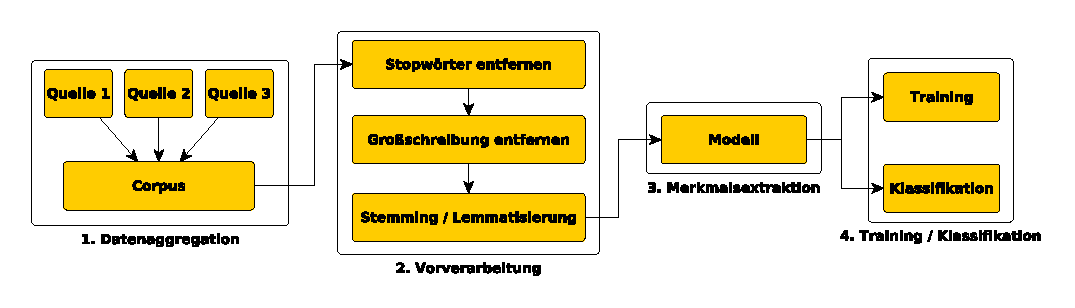
\includegraphics[scale=.80]{images/classification_pipeline_horizontal}
            \caption{Einzelschritte der Textklassifikation}\label{fig:pipeline}
        \end{figure}

        Der folgende Abschnitt beschreibt, wie die einzelnen Teilschritte der Pipeline im Rahmen dieser Seminararbeit implementiert wurden.

        \subsubsection{Datenaggregation}
            Zum Trainieren und Testen des Klassifikators werden Daten aus dem NLTK Brown Corpus verwendet. Darin enthalten sind Sätze verschiedener Themengebiete, welche als Liste einzelner Wörter vorliegen. 

            Die Implementierung des Klassifikators akzeptiert Daten in diesem Format, somit müssen keine weiteren Verarbeitungsschritte zur Datenaufbereitung vorgenommen werden.

        \subsubsection{Vorverarbeitung}
            Bevor Merkmale aus den Daten extrahiert werden, durchlaufen sie einen Vorverarbeitungsschritt, der die Eingangsdaten filtert und aufbereitet. 
            Dies geschieht in der vorliegenden Implementierung mit Hilfe der Klasse \textit{Preprocessor}, welche folgende Aufgaben übernimmt:\newline\newline
            \textbf{Stopwörter entfernen}:\newline
            Elemente natürlicher Sprache lassen sich bezüglich ihres Informationsgehalts unterscheiden. 
            Viele so genannte ``Füllwörter'' treten häufig auf, liefern allerdings keinen Mehrwert an Information bezüglich der Bedeutung eines Satzes bzw. Textes. 
            Da diese Füllwörter den Merkmalsraum eines Dokuments unnötig vergrößern, werden sie im Allgemeinen vor der Klassifikation entfernt~\cite{nltk}. 
            Die NLTK-Bibliothek beinhaltet zu diesem Zweck Wörterbücher mit Füllwörtern verschiedener Sprachen, welche in der Methode \textit{remove\_stopwords} verwendet werden, um diese aus den Daten zu entfernen.\newline\newline
            \textbf{Lemmatisierung}:\newline
            Durch Lemmatisierung wird versucht, die unterschiedlich gebeugten Formen eines Wortes in einem Dokument auf ihr Lemma zurückzuführen, um eine unnötige Vergrößerung des Merkmalsraumes zu vermeiden~\cite{IIR}.

            Dies wird mit Hilfe des in NLTK enthaltenen \textit{WordNetLemmatizer} erreicht, welcher sich in \textit{nltk.stem.wordnet} befindet und auf Daten von WordNet zurückgreift.\newline\newline
            \textbf{Interpunktion entfernen}:\newline
            Die in NLTK enthalten Daten beinhalten neben einzelnen Wörtern auch vollständige Interpunktion. 

            Da die unabhängig von der Dokumentenklasse häufig auftretenden Satzzeichen die Liste der für eine Klasse signifikanten Merkmale verfälschen würden, werden Merkmale, die in \textit{string.punctuation} enthalten sind, entfernt.\newline\newline
            \textbf{Großschreibung entfernen}:\newline
            Die Datensätze in \textit{nltk.corpus.brown.tagged\_sents} liegen in korrekter Groß- und Kleinschreibung vor. 
            Da für die Klassifikation nach Themengebiet die Groß- und Kleinschreibung keine signifikante Rolle spielt, werden die Eingangsdaten im Prozess der Vorverarbeitung auf Kleinschreibung vereinheitlicht.

        \subsubsection{Merkmalsextraktion}
                Nachdem die Eingangsdaten erfolgreich vorverarbeitet wurden, können im Schritt der Merkmalsextraktion klassifizierbare Merkmale daraus extrahiert werden. 
                Dabei wird mittels eines Sets ein Vokabular der Trainingsdaten erstellt (siehe Abschnitt~\ref{sec:vocab}), welches zur Erstellung der Merkmalsvektoren verwendet wird.

        \subsubsection{Training / Klassifikation}
                Im letzten Schritt der Pipeline wird nun entweder ein neuer Klassifikator anhand der aus Dokumenten extrahierten Merkmale trainiert, oder eben diese Dokumente werden mittels eines bereits trainierten Klassifikators klassifiziert. 
                
                Das prinzipielle Vorgehen dabei ist in Abbildung~\ref{fig:algo} dargestellt.

        \begin{figure}[htpb]
            \centering
            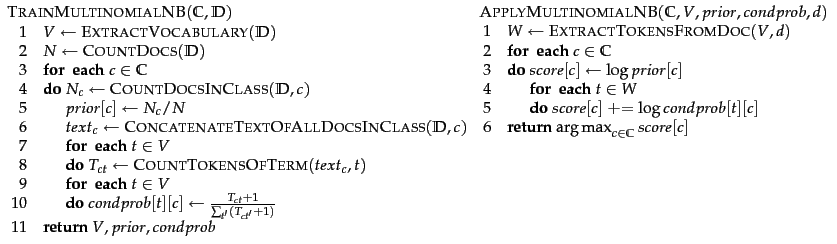
\includegraphics[scale=0.5]{images/algo2.png}
            \caption{Algorithmen für Training und Klassifikation\newline\tiny{Quelle: http://nlp.stanford.edu/IR-book/html/htmledition/naive-bayes-text-classification-1.html}}\label{fig:algo}
        \end{figure}

    \subsection{Arithmetischer Unterlauf}\label{sec:log}
    Anhand von Gleichung~\ref{eq:cond_prod} lässt sich erkennen, dass die bedingte Wahrscheinlichkeit $\hat{P}(\mathbf{x}|c)$ ein Produkt mehrerer Wahrscheinlichkeiten mit Werten im Bereich $0 \le x \le 1$ ist.

    Aufgrund der endlichen Genauigkeit der Gleitkommadarstellung von Computern kann es hierbei allerdings zu einem arithmetischen Unterlauf kommen und $\hat{P}(\mathbf{x}|c)$ wird zu $0$ gerundet. Um dieses Problem zu umgehen, bietet es sich an, mit logarithmierten Wahrscheinlichkeiten zu arbeiten~\cite{IIR}.
        
        Dadurch ergibt sich Gleichung~\ref{eq:class_bayes_3} zu:

        \begin{equation}
            c_{m} = \argmax_{c \in K}\left[\log{\hat{P}(c)} + \sum_{i=1}^{n}\log{\hat{P}(x_{i}|c)}\right]
            \label{eq:log_bayes}
        \end{equation}

    \subsection{Additive Smoothing}
    Eine ähnliche Problemstellung zu Abschnitt~\ref{sec:log} ergibt sich, wenn im Trainingsdatensatz ein Merkmal enthalten ist, das explizit nur in einer Dokumentenklasse~$c_{k}$ auftritt. Dieses Merkmal hätte somit in allen anderen Dokumentenklassen eine Wahrscheinlichkeit $\hat{P}(x_{i}|c = \neg c_{k}) = 0$.

        Dies hätte zur Folge, dass, ausgehend von Gleichung~\ref{eq:class_bayes_3}, das Produkt~\ref{eq:cond_prod} nur für Dokumentenklasse~$c_{k}$ ein Ergebnis ungleich~$0$ liefern würde und somit~$c_{k}$ stets als passendste Dokumentenklasse gewählt wird~\cite{IIR}.

        %Bei Verwendung von Gleichung~\ref{eq:log_bayes} hingegen würde der Ausdruck~$\log{(0)}$ ausgewertet werden, welcher nicht definiert ist.

        Um dieses Problem der ``Nullwahrscheinlichkeiten'' zu eliminieren, wird häufig sogenanntes ``additive smoothing'' angewandt.
        Dabei wird ein beliebiger Wert $\epsilon$ zur Anzahl des Vorkommens eines Merkmals addiert, um damit das Auftreten einer Nullwahrscheinlichkeit zu verhindern.

        Gleichung~\ref{eq:cond_prob_xi} ändert sich dadurch zu:

        \begin{equation}
            \hat{P}(x_{i}|c) = \frac{\left[\sum_{\mathbf{x} \in c}\sum_{x_{i} \in \mathbf{x}}1\right]+\epsilon}{\sum_{\mathbf{x} \in c}\left[\sum_{w \in \mathbf{x}}1+\epsilon\right]}
            \label{eq:add_one}
        \end{equation}

    \subsection{Evaluation}
        Um die Genauigkeit des implementierten Klassifikators zu ermitteln, wird mit Hilfe der Klasse \textit{Evaluator} eine k-fache Kreuzvalidierung durchgeführt. 

        Die durchschnittliche Genauigkeit des Klassifikators, welche durch eine 5-fache Kreuzvalidierung mit Daten der Kategorien \textit{humor} und \textit{learned} ermittelt wurde, beträgt dabei 88\%.

\section{Fazit}
    Anhand dieser Arbeit wurden die theoretischen Grundlagen des naiven Bayes-Klassifikators erarbeitet, sowie die Implementierung eines Klassifikators behandelt. 
    Dadurch ließ sich erkennen, dass sich ein Bayes-Klassifikator leicht implementieren lässt und mit 88\% Genauigkeit gute Ergebnisse liefert.

    Durch die Verwendung eines Vektorraummodells mit z.B. tf-idf Werten~\cite{IIR}, anstatt des in der vorliegenden Implementierung verwendeten Unigram-Wortsequenz-Modells, ließe sich die Genauigkeit des Klassifikators womöglich noch verbessern.

    %Da das verwendete Unigram-Wortsequenz-Modell stark von der Länge der einzelnen Dokumente abhängt, liese sich die Genauigkeit der Klassifikation eventuell durch die Verwendung eines Vektorraum-Modells verbessern.

\newpage
% literatur.tex
% (c) Simon Hofmann
% mail@simon-hofmann.org

%------ bibtex ------
\addcontentsline{toc}{section}{Literatur}
\bibliography{bib/library}
\bibliographystyle{plain}


% ---- Beim Erstellen der .tex files in den Editoroptionen UTF-8 als Zeichenkodierung verwenden

\end{document}
